In this chapter, we explore two different scenarios that can be achieved by the visualization application. The first demonstrates the influence of the mining strategy, and the second scenario shows the influence of network delay to the visualization. In addition, the presentation of orphaned blocks and forks proves that the visualization application handles the mining processes correctly. In the last scenario, we explore the limitation of the visualization application.

\section{Scenario I: Influence of Mining Strategy}

In the first scenario, there is a miner who has more chances to mine blocks than the other miners due to the mining strategy. With the low network delay, miners can publish the blocks quickly. Therefore, the miner who chooses the fastest mining strategy has more chances to win this game.

In this experiment, there are three miners, Alice (red color), Bob (blue color), and Charlie (green color), who compete with each other in the blockchain system. The configuration of this experiment is provided in Listing \ref{lst:scenario 1}.

As the configuration file shows, Alice's mining strategy is the fastest because the parameters of \textit{minimum value of transactions} and \textit{number of mined transactions} are all set to the lowest. On the contrary, Bob's parameter of \textit{number of mined transactions} and Charlie's parameter of \textit{minimum value of transactions} are higher than Alice's parameters. Therefore, the set of transactions that Alice can select is the largest.

The network delay is low. Hence, the blockchain network is stable and fast. (see Table \ref{tab:the parameters of the mining strategy in scenario I})

\begin{table}[htb]
    \centering
    \begin{subtable}{\textwidth}
        \centering
        \begin{tabular}{ M{8cm}|M{2cm} } 
            \hline
            \multicolumn{2}{c}{\textbf{Alice's Mining Strategy}} \\
            \hline
            \textit{Strategy Name} & \multicolumn{1}{c}{\textit{Value}} \\
            \hline
            Mining Time & 3 \\ 
            Minimum Value of Transactions & 1 \\ 
            Number of Mined Transactions & 1 \\
            \hline
        \end{tabular}
    \end{subtable}
    \begin{subtable}{\textwidth}
        \centering
        \begin{tabular}{ M{8cm}|M{2cm} } 
            \hline
            \multicolumn{2}{c}{\textbf{Bob's Mining Strategy}} \\
            \hline
            \textit{Strategy Name} & \multicolumn{1}{c}{\textit{Value}} \\
            \hline
            Mining Time & 3 \\ 
            Minimum Value of Transactions & 1 \\ 
            Number of Mined Transactions & 3 \\
            \hline
        \end{tabular}
    \end{subtable}
    \begin{subtable}{\textwidth}
        \centering
        \begin{tabular}{ M{8cm}|M{2cm} } 
            \hline
            \multicolumn{2}{c}{\textbf{Charlie's Mining Strategy}} \\
            \hline
            \textit{Strategy Name} & \multicolumn{1}{c}{\textit{Value}} \\
            \hline
            Mining Time & 3 \\ 
            Minimum Value of Transactions & 8 \\ 
            Number of Mined Transactions & 1 \\
            \hline
        \end{tabular}
    \end{subtable}
    \caption{The parameters of the mining strategy in scenario I.}
    \label{tab:the parameters of the mining strategy in scenario I}
\end{table}

Figure \ref{fig:alice was a fast miner} demonstrates the results of the above configuration. Although Bob and Charlie try to compete with Alice, she still dominated the blockchain system because of her fast mining strategy. As a result, most of the reward is won by Alice. 

\begin{figure}[htb]
    \centering
    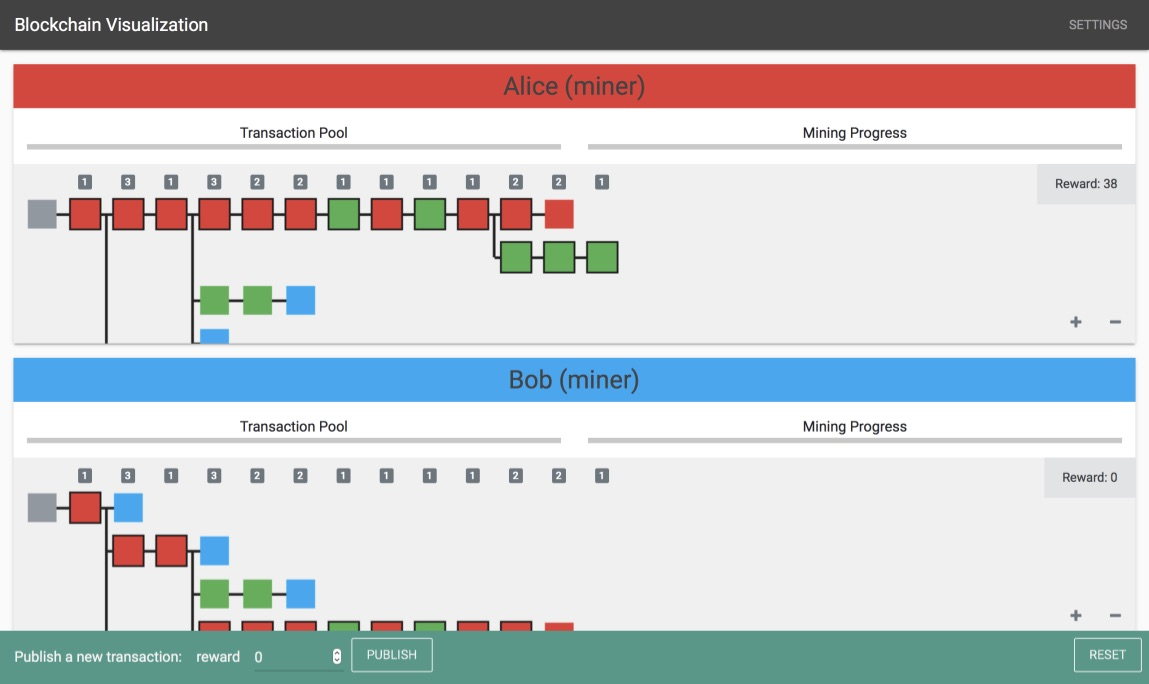
\includegraphics[width=\textwidth]{scenario_case1_2}
    \caption{Alice was a fast miner.}
    \label{fig:alice was a fast miner}
\end{figure}

\clearpage

In summary, this scenario shows the competition between the miners. As our expectation, the mining strategy with the lowest \textit{minimum value of transactions} and \textit{number of mined transactions} is the fastest one. Additionally, it shows that the orphaned blocks were handled by the visualization application correctly, as the fastest miner still worked on the correct blockchain data structure.

\section{Scenario II: Multiple Forks}

In the second scenario, there are four miners who are partitioned into two groups. Because the spread of blocks has high delay between different groups, miners in the same group add their own blocks to the blockchain much more quickly than other groups do. Thus, each group considers their own blockchain is the longest one, and the competition continues. Listing \ref{lst:scenario 2} is the configuration file for this scenario. 

In the configuration file, Alice and Bob are in the same group, and Charlie and David are in another group. Therefore, it is expected that there will be two forks because there are two partitioned groups. The parameters of the network delay between different groups are higher than the parameters of \textit{mining time} to simulate the bad network conditions. (see Table \ref{tab:the parameters of the mining strategy and the network delay in scenario II})

\begin{table}[htb]
    \centering
    \begin{subtable}{\textwidth}
        \centering
        \begin{tabular}{ M{8cm}|M{2cm} } 
            \hline
            \multicolumn{2}{c}{\textbf{Miner's Mining Strategy}} \\
            \hline
            \textit{Strategy Name} & \multicolumn{1}{c}{\textit{Value}} \\
            \hline
            Mining Time & 1 to 2 \\ 
            \hline
        \end{tabular}
    \end{subtable}
    \begin{subtable}{\textwidth}
        \centering
        \begin{tabular}{ M{8cm}|M{2cm} } 
            \hline
            \multicolumn{2}{c}{\textbf{Network Delay}} \\
            \hline
            \textit{Strategy Name} & \multicolumn{1}{c}{\textit{Value}} \\
            \hline
            In the same group & 1 \\ 
            Between different groups & 7 to 10 \\ 
            \hline
        \end{tabular}
    \end{subtable}
    \caption{The parameters of the mining strategy and the network delay in scenario II.}
    \label{tab:the parameters of the mining strategy and the network delay in scenario II}
\end{table}

\begin{figure}[htb]
    \centering
    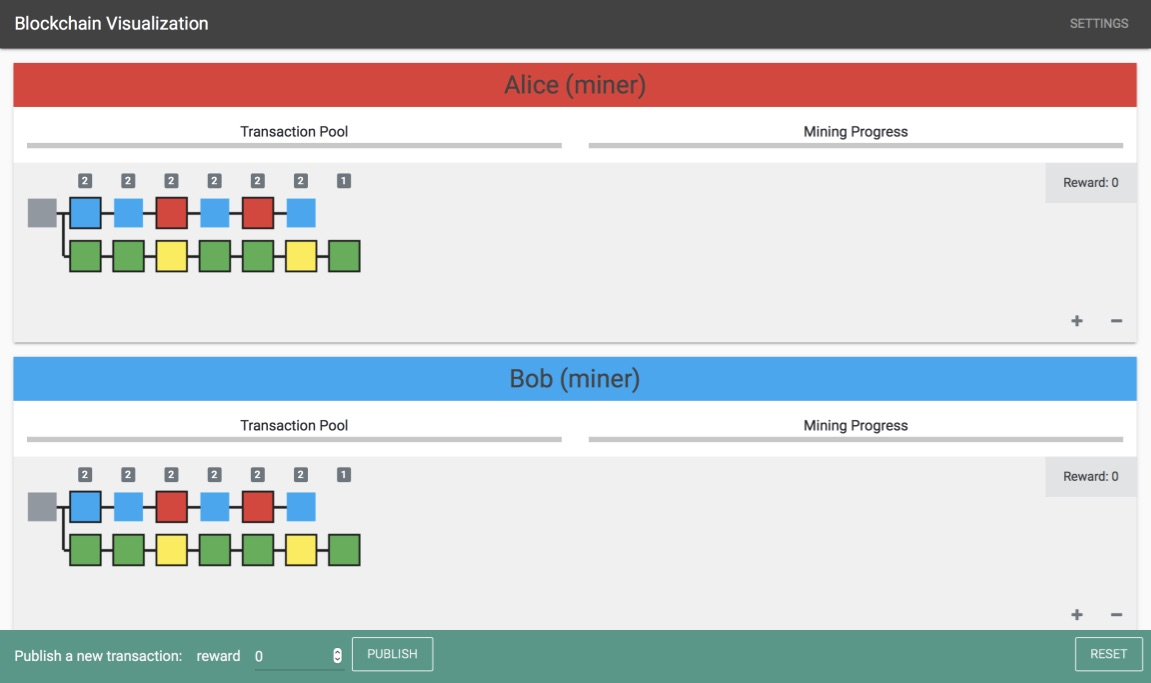
\includegraphics[width=\textwidth]{scenario_case2_5}
    \caption{Alice, Bob, and Charlie competed with each other.}
    \label{fig:alice, bob, and charlie competed with each other}
\end{figure}

In Figure \ref{fig:alice, bob, and charlie competed with each other}, the two groups compete with each other for a long time because the duration of mining time is shorter than the duration of publishing blocks. The miners are divided into two groups which work on different blockchain data structures because every group considered that their own blockchain is the longest. It can be checked that the mining processes visualized the mining processes according to the above description.

In conclusion, it demonstrates that the visualization application is influenced by the network delay. Furthermore, the forks during the mining processes are also correct. However, there is a weak point in the visualization application. The forks cannot be merged in the current implementation because the parameters of the mining strategy are fixed during the visualization. Thus, the scenario of multiple forks in the visualization represents the case of the hard forks in the real blockchain networks. It should be improved to handle the case of the soft forks in the future.

\section{Limitation of Nodes and Transactions}

Through experiments, we found that the maximum number of nodes that can be handled by the application is 15 because of the limitation of the visualization engine, i.e., the Three.js library. The visualization engine cannot create too many canvases due to the performance issue. Hence, the sum of the number of miners and nonminers is limited to 15. On the other hand, the number of transactions that can be handled should be unlimited. We tested it by publishing 100 transactions, and the application still operates correctly. Figure \ref{fig:result of the limitation experiment} shows the result of this experiment.

\begin{figure}[htb]
    \centering
    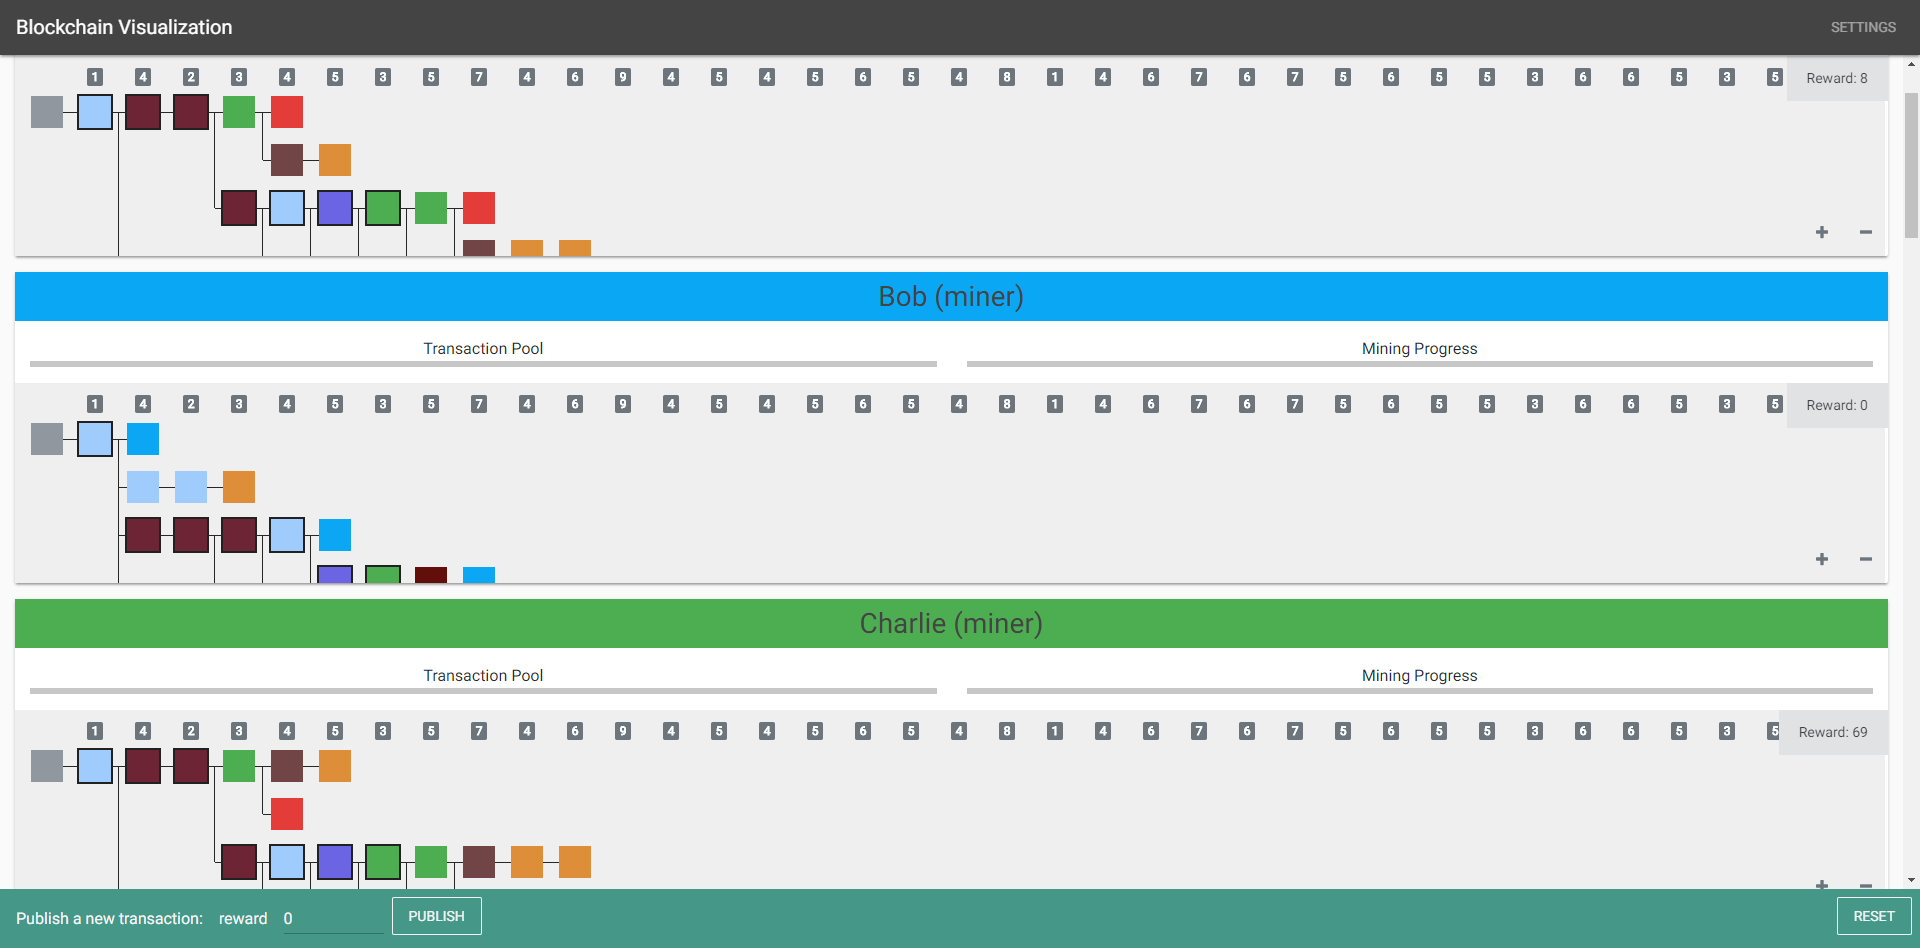
\includegraphics[width=\textwidth]{scenario_case3}
    \caption{Result of the limitation experiment.}
    \label{fig:result of the limitation experiment}
\end{figure}

